% !TeX root = ../../thesis.tex

\section{\acs{UEFI} Shell}

% try in EFI shell
% what is the EFI shell
\TODO{better summary of UEFI shell}
Part of the family of \ac{UEFI} specifications is a shell specification which defines a feature rich \ac{UEFI} shell application to interact with the \ac{UEFI} environment \cite[Section 1.1]{uefi-shell-spec}.
It offers commands related to boot and general configuration, device and driver management, file system access, networking \cite[Section 5.1]{uefi-shell-spec} and supports scripting \cite[Section 4]{uefi-shell-spec}.

The \ac{UEFI} shell may already be part of the boot options but can always be supplied on a \ac{USB} stick in the default boot path.
\autoref{fig:uefi-shell} depicts an exemplary output of an \ac{EDK} II \ac{UEFI} shell emulated under QEMU.
steal me from neither


Upon invocation, the shell application performs an initialization during which it \TODO{does what? whats important for us here} and produces output what is equivalent to the output of the execution of the commands \lstinline{ver} and \lstinline{map -terse} \cite[Section 3.3]{uefi-shell-spec}.
\lstinline{ver} displays the version of the \ac{UEFI} specification the firmware conforms to \cite[Section 5.3]{uefi-shell-spec}.


% showing mapping, also available with map command
% consistent device mapping, comparable to partition names in windows
The map command is very interesting for file access with the shell, it displays a mapping table between user defined alias names and device handles.
The aliases can be used instead of a device path when submitting commands via the command line interface.
The \ac{UEFI} shell also produces default mappings, notably for file systems \cite[Section 3.7.2]{uefi-shell-spec}.
These mappings are designed to be consistent across reboots as long as the hardware configuration stays the same, they are comparable to Windows partition letters \cite[Appendix A]{uefi-shell-spec}.

\TODO{find in spec what precise mapping mechanism}
When we inspect the mapping table we can see \lstinline{FSx:} and \lstinline{BLKx:} aliases, \lstinline{FSx:} maps to file systems and \lstinline{BLKx:} to block devices.
This identification is performed via instances of the \hyperref[lst:simple-file-system-protocol]{Simple File System Protocol} and \TODO{double check} Block \ac{I/O} Protocol.
% explain Simple File System Protocol
The \hyperref[lst:simple-file-system-protocol]{Simple File System Protocol} \cite[Section 13.4]{uefi-spec} provides, together with the \hyperref[lst:simple-file-system-protocol]{File Protocol}, file-type access to the device it is installed on \cite[Section 13.5]{uefi-spec}.
The two protocols are independent of the underlying file system the media is formatted with.



\TODO{me}

\begin{figure}[htb]
    \centering
    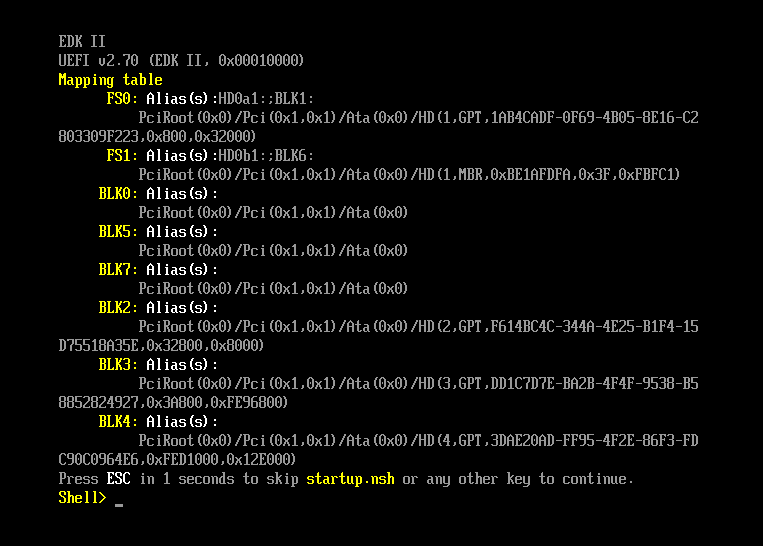
\includegraphics[width=1.0\textwidth]{uefi_shell.png}
    \caption{\ac{UEFI} command prompt}
    \label{fig:uefi-shell}
\end{figure}
